%% LyX 2.0.3 created this file.  For more info, see http://www.lyx.org/.
%% Do not edit unless you really know what you are doing.
\documentclass[english]{article}
\usepackage[T1]{fontenc}
\usepackage[latin1]{inputenc}
\usepackage{float}
\usepackage{amstext}
\usepackage{amssymb}
\usepackage{graphicx}

\makeatletter

%%%%%%%%%%%%%%%%%%%%%%%%%%%%%% LyX specific LaTeX commands.
\newcommand{\lyxmathsym}[1]{\ifmmode\begingroup\def\b@ld{bold}
  \text{\ifx\math@version\b@ld\bfseries\fi#1}\endgroup\else#1\fi}

%% For printing a cirumflex inside a formula
\newcommand{\mathcircumflex}[0]{\mbox{\^{}}}

%% Because html converters don't know tabularnewline
\providecommand{\tabularnewline}{\\}
\floatstyle{ruled}
\newfloat{algorithm}{tbp}{loa}
\providecommand{\algorithmname}{Algorithm}
\floatname{algorithm}{\protect\algorithmname}

%%%%%%%%%%%%%%%%%%%%%%%%%%%%%% Textclass specific LaTeX commands.
 \usepackage{algolyx}

%%%%%%%%%%%%%%%%%%%%%%%%%%%%%% User specified LaTeX commands.
% Language
% \algolang{french}

% Algorithmic possible option
% \def\algoption{noend}

% Comments delimiters redefinition
% \keycomment{\#<}{>\#}

\makeatother

\usepackage{babel}
\begin{document}

\title{Modeling the Transport Equation for Cosmic Strings}


\author{Jacob Balma, Daniel Schubring, Vitaly Vanchurin}
\maketitle
\begin{abstract}
This documentation prescribes an algorithm for modeling the transport
equation for cosmic strings as proposed by V. Vanchurin and D. Schubring
in {[}3{]}. We use Lebedev Quadrature as our method of numerical integration. 

\tableofcontents{}

\newpage{}
\end{abstract}

\section*{Introduction}

We would like to study numerically how a distribution of strings with
both longitudinal and transverse collisions goes to equilibrium under
various expanding backgrounds. For an introduction to Cosmic Strings,
see {[}7{]}. This document will be organized as follows. In part I,
we introduce the Transport Equation for interacting Nambu-Goto strings,
and prescribe an algorithm to model the collision terms. In Part II,
we introduce the gravitational term, and a technique for calculating
its components. In part III we introduce a method of loop removal
and present results.


\section{Transport Equation}

\begin{equation}
\frac{df}{dt}=\left(\frac{df}{dt}\right)_{collision}+\left(\frac{df}{dt}\right)_{spatial}+\left(\frac{df}{dt}\right)_{gravitational}
\end{equation}


The transport equation:\medskip{}


\[
\left(\frac{df(\mathbf{A},\mathbf{B})}{dt}\right)_{spatial}+\left(\frac{d}{dt}+\mathcal{H}\left(\partial_{A}+\partial_{B}-(1+\mathbf{A}\cdot\mathbf{B})-4(\mathbf{A}\cdot\mathbf{B})\right)\right)f(\mathbf{A},\mathbf{B})=
\]


\begin{equation}
\frac{1}{\rho}\int\, d\mathbf{A}'d\mathbf{B}'\,\Gamma\left(\, f(\mathbf{A}',\mathbf{B})f(\mathbf{A},\mathbf{B}')-f(\mathbf{A},\mathbf{B})f(\mathbf{A}',\mathbf{B}')\,\right)
\end{equation}


More detail can be found on the spatial term in {[}Ref. 3, Eq. 5.5{]}.
For the purposes of this paper, we will focus on the the collision
and gravitational terms respectively.\textbf{ A} and \textbf{B} are
unit three-vectors on the sphere and correspond to tangent vectors
of right and left moving waves. We can also define the quantities
\textbf{u} and \textbf{v}, which are also unit vectors that correspond
to longitudinal and transverse velocities for string segments.

\[
\mathbf{v}=\frac{\mathbf{A}+\mathbf{B}}{2}
\]
\[
\mathbf{u}=\frac{\mathbf{B}-\mathbf{A}}{2}
\]


And since \textbf{u} and \textbf{v} can both be written in terms of
\textbf{A} and \textbf{B}, this says that if \textbf{A}=-\textbf{B},
then the propagation is all along \textbf{u}. Likewise, if \textbf{A}=\textbf{B},
then \textbf{u}=0 and everything is along \textbf{v}. 

\medskip{}


In the homogeneous limit, and ignoring gravitational effects, the
localized transport equation reduces to just the right hand side,
which is the collision term from (1):

\begin{equation}
\left(\frac{df}{dt}\right)_{collision}=\left(\frac{df}{dt}\right)_{transverse}+\left(\frac{df}{dt}\right)_{longitudinal}
\end{equation}


\medskip{}


\begin{equation}
\left(\frac{df}{dt}\right)_{collision}=\frac{1}{\rho}\int\, d\mathbf{A}'d\mathbf{B}'\,\Gamma\left(\, f(\mathbf{A}',\mathbf{B})f(\mathbf{A},\mathbf{B}')-f(\mathbf{A},\mathbf{B})f(\mathbf{A}',\mathbf{B}')\,\right)
\end{equation}


\medskip{}


So to start out, we are going to model the collision term on its own.
As we can see from (4), we must integrate over \textbf{$\mathbf{A}'$}
and \textbf{$\mathbf{B}'$}, which are unit vectors on the sphere
and correspond to right and left moving tangent vectors. They depend
on two coordinates. The azimuthal angle $\phi$, and polar angle $\theta$. 


\subsection{Lebedev Quadrature}

Naively, solving (4) numerically, involves four integrals at each
time step because \textbf{A} and \textbf{B} have two components each,
which implies we have four nested loops (one for each component).
But a numerical integration technique known as quadrature will help
us to improve upon this. This is an important step, so some time will
be spent ensuring you understand the technique and benefits of using
it. Lebedev quadrature gives an approximation to the surface integral
of a function over the sphere. When using Lebedev Quadrature, the
distribution of points on the sphere (the points where your function
is evaluated) have octahedral symmetry, which means the location of
the points remain invariant under certain types of transformations.
In addition, the points are relatively evenly distributed. Quadrature
requires only one summation to perform a 2-dimensional integral, although
the number of iterations required would be the same as the naive approach.
The main benefit is that the distribution of points does not bunch
up near the poles, as in the naive approach. The technique also allows
for exact integration of spherical harmonics, which will be extremely
useful when evaluating the gravitational terms.

The core of this technique comes from a set of points on the sphere
and corresponding weights for each point. These are known as ``rules'',
and Vyacheslav Lebedev computed many of them using an algebraic method
in the late seventies. So techniques exist for computing them on your
own, but in the end you will end up with a list of points and corresponding
weights. John Burkardt from Florida State University has been so kind
as to provide individual text files ranked in order of precision (the
maximum order of the polynomial evaluated) referenced in {[}5{]}.
My advice would be download them and use which ever order of precision
you find necessary. A rule of precision p can be used to correctly
integrate any polynomial for which the highest degree term $x^{i}y^{j}z^{k}$
satisfies $i+j+k\leq p$. For example, a polynomial with i+j+k=3 has
precision 3 and requires 6 points to correctly integrate. Higher precision
requires a higher number of points, and in turn, requires more time
to integrate. Thus the level of precision you choose is limited by
the computational resources available. But the types of functions
you wish to integrate may be sensitive to this precision as well.
The level of precision is a side-note at this point, but will be discussed
in more detail as we move on to discuss the gravitational terms in
Part III.

When we integrate a function $f(\theta,\phi)$ over the surface of
the unit sphere, we expect to get a number, a.

\[
a=\intop_{0}^{2\pi}\,\intop_{0}^{\pi}\, f(\theta,\phi)\, sin(\theta)\, d\theta\, d\phi
\]


The naive approach would be to take interval of your coordinates and
split them up into N pieces that correspond to the step-size, $\Delta x=1/N$.
You then make an array of your coordinates over which you are integrating
and plug those into your function as you sum it up N times, multiplying
by step size each iteration. The naive approach yields two summations
for an integral in spherical coordinates on a unit sphere:

\[
a=\sum_{i=0}^{N}\sum_{j=0}^{M}f(\theta_{i},\phi_{j})sin(\theta_{i})\Delta\theta\Delta\phi
\]


where 
\[
\Delta\theta=\frac{\pi}{N}
\]


\[
\Delta\phi=\frac{2\pi}{M}
\]


The other facet of the naive approach is the fact that near the poles
of the unit sphere, there are more ``pieces'' and hence more time
is spent evaluating these parts of a function. Quadrature is a little
different. We still require the list of coordinates (provided by the
rule you choose), only now we multiply by the weight each iteration.
These weights will be different depending on the location of the point,
as opposed to the naive approach where $\Delta x$ is constant. It
allows us to give the same amount of computation time to points near
the poles as we would of points around the azimuth. We can think of
this as a way of making the points we evaluate the function at as
being equidistant apart.

But before we get to the algorithm needed to perform Lebedev Quadrature,
we need to develop a way to access the points and their corresponding
weights. The first thing our algorithm requires is a ``Point'' object.
This object has an important role to play. It will be a container
for the file which contains the Lebedev points and their weights.
Ideally, we would like to use an array of Point objects, each representing
a specific point on the sphere. It should have a few basic functions
built in: One for setting the coordinates of a particular point and
its weight, and three for retrieving each individual component. If
you have n points to store, then this should work:

\begin{algorithm}[!h]
\begin{algor}
\item [{for}] \ensuremath{(i=0;\, i<N;\, i++)}


\begin{algor}
\item [{{*}}] $infile(theta[i],phi[i],weight[i])$\{fill arrays with$\theta_{i}$,$\phi_{i}$,$w_{i}$
from 3-column data file\}
\item [{{*}}] $Point[i].SetTheta(theta[i])$
\item [{{*}}] $Point[i].SetPhi(phi[i])$
\item [{{*}}] $Point[i].SetWeight(weight[i])$
\end{algor}
\item [{endfor}]~
\end{algor}
\caption{Read in weight and coordinate data from file}
\end{algorithm}


Note that the above algorithm treats the first column as the $\theta$-coordinate
(i.e. the polar angle), and the second column as the $\phi$-coordinate
(i.e. the azimuthal angle). John Burkardt's rules treat these columns
in the opposite way. Column one is labelled $\phi\epsilon[0,\pi]$
and column two is labelled $\theta\epsilon[-\pi,\pi]$ such that the
traditional formulae used to convert between Spherical and Cartesian
coordinate systems swap z=cos(theta) for z=cos(phi), as well as the
coordinates in the formula for x and y. In this documentation, and
the code referenced in {[}6{]}, we will be treating column one as
$\theta\epsilon[0,2\pi]$, and column two as $\phi\epsilon[-\pi,\pi]$.
Graphically this is what you would expect.

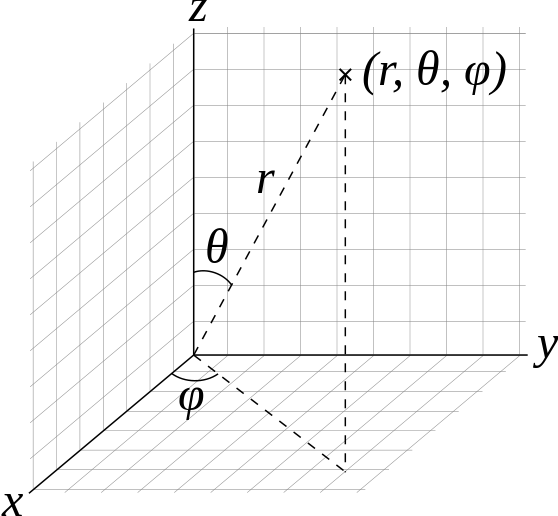
\includegraphics[scale=0.25]{coordinates}

Where the Cartesian coordinates are given by,

$x=sin(\theta)cos(\phi)$

$y=sin(\theta)sin(\phi)$

$z=cos(\theta)$

What you call theta and phi are determined only by preference, but
care must be taken to be completely consistent in these preferences
when defining your vector math, as well as the Spherical Harmonic
functions used later. \pagebreak{}

Now, we are ready to integrate some functions. The format to integrate
using the Lebedev Quadrature goes like,

\begin{equation}
a=\sum_{i=0}^{n}\,4\pi\, f(\theta_{i},\phi_{i})w_{i}
\end{equation}


\begin{algorithm}[!h]
\begin{algor}
\item [{for}] \ensuremath{(i=0;\, i<N;\, i++)}


\begin{algor}
\item [{{*}}] $a=a+4\pi f(Point[i].GetTheta())\, f(Point[i].GetPhi())\, Point[i].GetWeight()$ 
\end{algor}
\item [{endfor}]~
\end{algor}
\caption{General integration using Lebedev Quadrature}
\end{algorithm}


Where $w_{i}$ is the weight corresponding to the two points. Notice
there is no sine function here as would normally appear when integrating
in spherical coordinates. We also have a factor of $4\pi$ out front.
This implies that summing over the weights should sum to one, which
they do. So that is a good first test. Adding the constant factor
out front gives the correct surface area of a unit sphere. Now try
integrating $f(\theta,\phi)=x^{2}y^{2}z^{2}$. This is a spherical
harmonic. It should evaluate exactly. Recalling the rule for integration
using the Lebedev Quadrature, $i+j+k\leq p$, p must be at least 6.
Therefore the minimum number of points we can use for the function
to evaluate exactly is 26, with a precision of 7. The function should
come out to be $\frac{4\pi}{105}\approx0.11968$. Algorithmically,
we have:

\[
a=\sum_{i=0}^{n}\,4\pi\, sin(\theta_{i})^{4}cos(\theta_{i})^{2}sin(\phi_{i})^{2}cos(\phi_{i})^{2}w_{i}
\]


\begin{algorithm}[!h]
\begin{algor}
\item [{for}] \ensuremath{(i=0;\, i<N;\, i++)}


\begin{algor}
\item [{{*}}] $a=a+4\pi\, sin(Point[i].GetTheta())^{4}cos(Point[i].GetTheta())^{2}$ 
\item [{{*}}] $sin(Point[i].GetPhi())^{2}cos(Point[i].GetPhi())^{2}Point[i].GetWeight()$
\end{algor}
\item [{endfor}]~
\end{algor}
\caption{Integrate $f(\theta,\phi)=x^{2}y^{2}z^{2}$}
\end{algorithm}


If you use the appropriate rule, the function will evaluate exactly
as you would expect. However, what happens if you choose the prior
set of points (p=5, with 14 points)? We get an answer over twice our
expectation, $a\thickapprox0.279253$. Cleary taking care to use a
precision high enough to deal with the polynomial evaluated is important.

Now let's try a function which is not a spherical harmonic, $f(\theta,\phi)=cos\left(\theta\right)^{4}sin(\phi)^{4}$. 

\[
a=\sum_{i=0}^{n}\,4\pi\, cos\left(\theta\right)^{4}sin(\phi)^{4}w_{i}
\]


It should integrate to $\frac{3\pi}{10}$. Here you will notice a
sensitivity to the number of points used because this function is
not a spherical harmonic. When calculated using a rule of 11 (50 Points),
we are within 92.9\% of the correct value, but it's not exact. Using
a rule with precision 17 (110 points) yields a result within 99.7\%.
Burkardt provides rules for precisions all the way up to 131 (5810
Points), but these will be outside the computational feasibility for
our task. Most likely we will be operating between 26 and 110 points
because most of the functions we will be dealing with will be spherical
harmonics and therefore will be easy to evaluate using this method.
Numerically this provides a good trade-off for speed while not sacrificing
much accuracy. Now armed with our integration technique, we are ready
to simulate the collision terms.


\subsection{Numerical Transport Equation Collision Term}

Recall that the collision terms evolve according to (4). Moving dt
to the right hand side gives the rule for evolution at each time step
$\triangle t$:

\begin{equation}
\left(df(\mathbf{A},\mathbf{B})\right)_{col}=\frac{1}{\rho}\int\, d\mathbf{A}'d\mathbf{B}'\,\Gamma\left(\, f(\mathbf{A}',\mathbf{B})f(\mathbf{A},\mathbf{B}')-f(\mathbf{A},\mathbf{B})f(\mathbf{A}',\mathbf{B}')\,\right)dt
\end{equation}


where

\begin{equation}
\Gamma(A,B,A',B')=\lambda(\frac{1}{\mu})+\mu\rho pP(A,B,A',B')
\end{equation}


Both $\lambda$ and $p$ are probabilities. For now, we set both to
1, as well as the correlation length $\mu$. Later on we will calculate
$\mu$ dynamically. In terms of Lebedev Quadrature, we index over
arrays labeled by the points A,B,A', and B' such that equation 9 becomes:

\begin{equation}
\left(df(A,B)\right)_{col}=\sum_{A'=0}^{n}\sum_{B'=0}^{n}\frac{1}{\rho}\, w_{A'}w_{B'}\,\Gamma_{A,B,A',B'}\left(\, f(A',B)f(A,B')-f(A,B)f(A',B')\,\right)\Delta t
\end{equation}


The first step is to create a time loop. The time loop is an iterative
loop that goes from $t=t_{0}$ to $t=t_{max}$. Either of these constants
are arbitrary, which is a benefit of the statistical approach. Defining
$t_{max}\gg t_{0}$ so we have a long time to see if the system equilibrates.
Then we also define the proper time, $\tau$. This is a way of keeping
track of the time according to your step size, as opposed to the iterative
value of t. 

$T=t_{0}+t\,\triangle t$

The step size $\Delta t$ will be somewhat arbitrary, although you
will find that smaller step sizes allow you to probe finer details
of the system as it equilibrates. This is something you can set at
run-time. So your main loop has the form:

\begin{algorithm}[!h]
\begin{algor}
\item [{while}] $t<t_{max}$
\item [{do}] $\tau=t_{0}+t\,\Delta t$
\item [{{*}}] \{all calculations will go here\}
\item [{{*}}] t++
\item [{endwhile}]~
\end{algor}
\caption{Main time-loop}
\end{algorithm}


Everything we do from here on will take place within this loop.

Next we need to setup two arrays, one for df(\textbf{A},\textbf{B}),
and one for f(\textbf{A},\textbf{B}).

The first thing we need for this step is to setup a distribution function
$f(\mathbf{A},\mathbf{B})$. Luckily, the distribution function is
just a 2-d matrix that is a place a holder for what the evolution
does. It is indexed by the Lebedev points. So we simply need to define
an empty 2-dimensional array. The same goes for df(\textbf{A},\textbf{B}).
The integration takes place within one time step $\bigtriangleup t$.
We then update the matrix $f[A][B]$, and repeat the operation for
an arbitrary length of time $\tau$. When the system reaches equilibrium,
every component of df{[}A{]}{[}B{]} should be zero (to a close numerical
approximation).

Note that the iterators A, B, A', B' are simply integers that index
our matrices. We use this convention just to keep our notation clear.
The real coordinate values contained at a point come from our Point
object and the corresponding weight. We then put the entire integration
function inside the time loop.

Before we can model (8), we need to define a few more quantities.
First The normalization term comes from the energy density, $\rho$.
To calculate the energy density, simply integrate over the probability
density function f(A,B).

\begin{equation}
\rho=\int f(\mathbf{A},\mathbf{B})\, d\mathbf{A}\, d\mathbf{B}
\end{equation}


This is something that we now know how to do:

\[
\rho=\sum_{A}^{n}\sum_{B}^{n}f(A,B)w_{A}w_{B}
\]


\begin{algorithm}[!h]
\begin{algor}
\item [{for}] \ensuremath{(A=0;\, A<N;\, A++)}


\begin{algor}
\item [{for}] $(B=0;\: B<N;\: B++)$
\item [{{*}}] $\rho=\rho+f[A][B]\, Point[A].GetWeight()\, Point[B].GetWeight()$ 
\item [{endfor}]~
\end{algor}
\item [{endfor}]~
\end{algor}
\caption{Calculate the energy density using Lebedev Quadrature}
\end{algorithm}


The other term we need to define is from (7),$\Gamma(P,p)$. It depends
on the cross-sectional volume element P, and the inter-commutation
probability p. These terms tell us about the likelihood for strings
to interact on their world sheets (see {[}4{]}). The volume element
P contains wedge products (or a few dot and cross products) between
points on the sphere. In general, $\Gamma$ describes the rate of
interaction between string segments within the volume defined by P
due to transverse collisions. 

\[
P=|A\mathcircumflex B\mathcircumflex A'\mathcircumflex B'|
\]


\[
P\propto|(v'-v)\cdot(u'\times u)|=\frac{1}{8}|(A'+B'-A-B)\cdot((B'-A')\times(B-A))|
\]


The 1 in (7) corresponds to the probability of longitudinal collisions.
For now, this probability is unity, but it can be tweaked later on.
You could calculate $\Gamma$ directly in the inner-most loop using
some vector math, but that turns out to be computationally expensive.
Since the wedge product terms in P turn out to be a function of only
the Lebedev points, we can calculate it one time before we even start
the time loop, and then just index a 4-d array in which the values
have been stored. In fact, a good rule of thumb is to keep the inner-loop
as free of actual computation as possible. This means, do not call
functions within the inner loops. Instead, try to do actual computation
outside the loop and just store the values in an array to be iterated
over. It is much more efficient to just look at memory locations rather
than to call functions. This is true in C++ and likely the case in
any other object-oriented programming language.

\begin{algorithm}[!h]
\begin{algor}
\item [{for}] \ensuremath{(A=0;\, A<N;\, A++)}


\begin{algor}
\item [{for}] $(B=0;\: B<N;\: B++)$

\begin{algor}
\item [{for}] \ensuremath{(A=0;\, A<N;\, A++)}


\begin{algor}
\item [{for}] $(B=0;\: B<N;\: B++)$
\item [{{*}}] $P[A][B][A'][B']=(\frac{1}{8})\, abs(\,(Point[A']+Point[B']-Point[A]-Point[B])\,\circ\,$$((Point[B']-Point[A'])\times(Point[B]-Point[A]))\,)$ 
\item [{endfor}]~
\end{algor}
\item [{endfor}]~
\end{algor}
\item [{endfor}]~
\end{algor}
\item [{endfor}]~
\end{algor}
\caption{Store the wedge product terms to 4-d array}
\end{algorithm}


Here $\circ$ and $\times$ are taken to be the traditional dot and
cross products for three-vectors. This brings us to an important aside.
Your Point object should be capable of doing basic vector math. That
is, you need to define an overloaded operator, or some function which
computes cross and dot products by converting between spherical and
Cartesian coordinates. You should also have a way to do vector addition
and scalar multiplication. Later, we will also require that points
go back and forth between spherical and Cartesian coordinate systems.
So your Point object should have some additional functions, like GetX(),
GetY(), GetZ(). Using overloaded operators, you can also define a
wedge product such that the above code will be simplified further.
The ability to do vector math in a compact and intuitive way is very
helpful, but greatly depends on the language which you program in.
In C++, operator overloading is by far the superior method due to
its compactness. But one can use functions that perform the above
tasks just as quickly, or separate libraries like Boost, in which
you can call predefined functions for most vector and matrix math.

Now that we have defined P, we can iterate over the stored values
and set up our final integration step in modeling the collision terms. 

\[
\left(df(A,B)\right)_{col}=\sum_{A'=0}^{n}\sum_{B'=0}^{n}\frac{1}{\rho}\, w_{A'}w_{B'}\,(1+p\rho P(A,B,A',B'))\left(\, f(A',B)f(A,B')-f(A,B)f(A',B')\,\right)\Delta t
\]


\begin{algorithm}[!h]
\begin{algor}
\item [{for}] \ensuremath{(A=0;\, A<N;\, A++)}


\begin{algor}
\item [{for}] $(B=0;\: B<N;\: B++)$

\begin{algor}
\item [{for}] \ensuremath{(A=0;\, A<N;\, A++)}


\begin{algor}
\item [{for}] $(B=0;\: B<N;\: B++)$
\item [{{*}}] $df[A][B]=df[A][B]+(\frac{1}{\rho})\,(1+\rho pP[A][B][A'][B'])(f[A'][B]f[A][B']-f[A][B]f[A'][B'])\, Point[A'].GetWeight()\, Point[B'].GetWeight()\Delta t$ 
\item [{endfor}]~
\end{algor}
\item [{endfor}]~
\end{algor}
\item [{endfor}]~
\end{algor}
\item [{endfor}]~
\end{algor}
\caption{Calculate the collision term $\left(df(A,B)\right)_{col}$}
\end{algorithm}


Then, simply add the change due to collisions back into the distribution
function.

\begin{algorithm}[!h]
\begin{algor}
\item [{for}] \ensuremath{(A=0;\, A<N;\, A++)}


\begin{algor}
\item [{for}] $(B=0;\: B<N;\: B++)$

\begin{algor}
\item [{{*}}] $f[A][B]=f[A][B]+df[A][B]$ 
\end{algor}
\item [{endfor}]~
\end{algor}
\item [{endfor}]~
\end{algor}
\caption{Update the distribution}
\end{algorithm}


The time loop then starts over, and we repeat the operation.


\subsection{Initial Conditions}

Of course, the pseudo-code above will not do anything just yet because
we have not filled the distribution function array with any values.
We must fill f{[}A{]}{[}B{]} with initial conditions from which the
transport equation will determine the system's evolution. We need
an initial distribution function on the sphere such that we can easily
define a peak on the A and B spheres. This allows us to manipulate
the initial average u and v with which the system starts out with. 

In {[}4{]}, it was thought that the distribution function need to
be of a particular form. A probability distribution on the sphere
is called a Von-Mis Fisher distribution. It is basically a Gaussian
distribution peaked around some particular $(\theta,\phi)$ on the
unit sphere. However, you will find through numerical analysis that
any non-factorisable distribution on the sphere eventually goes to
equilibrium. Still the Von Mises-Fisher Distribution is extremely
useful in setting initial conditions because it allows you to control
the average direction velocities are peaked in. It is defined as:

\begin{equation}
VMF(A,B)=\frac{exp\left(\frac{a\cdot A}{\alpha}+\frac{b\cdot B}{\beta}\right)+\Gamma}{16\pi^{2}\alpha\beta sinh\left(\frac{1}{\alpha}\right)sinh\left(\frac{1}{\beta}\right)}
\end{equation}


This function is a non-factorisable normalized distribution on the
unit 4-sphere. It is non-factorisable due to the gamma term, which
was defined in equation 10 above. It contains the dot and cross product
terms. The mean directions are determined by \textbf{a} and\textbf{
b} on their respective spheres. For now, it suffices to say that non-factorisable
initial distributions eventually equilibrate, and factorisable initial
distributions are already in equilibrium. It's easiest to see what
is meant by factorisable by example:

\medskip{}


Factorisable: $e^{(x+y+z)}=f(x)f(y)f(z)$

Non-Factorisable: $e^{\left(xyz\right)}=f(x,y,z)$

\medskip{}


In Statistical Mechanics, proving a system equilibrates requires we
show that the distribution function (a distribution of velocities
in a volume element) factorizes after enough time has passed. That
is, we want to know whether a system that starts out as a big complicated
mess, eventually settles down to something where the original parameters
are no longer coupled. This obviously implies that systems in equilibrium
must be factorisable. For a system of particles that means $f(q,p)=f(q)f(p)$
in equilibrium. Intuitively, this just means that after a system has
reached equilibrium, the velocities of particles are not correlated
to their positions. There is an analogous conjecture for a distribution
of strings with velocities u(A,B) and v(A,B). We will study this further
in the next section. 


\subsection{H-Theorem}

The first thing we can do once we have a distribution function that
evolves according to a transport equation is prove an H-theorem for
strings, which is analogous to Boltzmann's H-theorem for particles.
This is the familiar notion that entropy of a system always increases.
Because H is simply entropy without the minus sign, it should always
decrease.

\[
H(t)=\int\, d\mathbf{A}\, d\mathbf{B}\, f(\mathbf{A},\mathbf{B})\, ln\left(f(\mathbf{A},\mathbf{B})\right)
\]


\[
\frac{d}{dt}H\leq0
\]


We see how H evolves numerically by evaluating the above integral
at each time step. Algorithmically, this is the same approach as we
took with the energy density integral:

\[
H=\sum_{A}^{n}\sum_{B}^{n}f(A,B)\, ln(f(A,B))\, w_{A}w_{B}
\]


\begin{algorithm}[!h]
\begin{algor}
\item [{for}] \ensuremath{(A=0;\, A<N;\, A++)}


\begin{algor}
\item [{for}] $(B=0;\: B<N;\: B++)$
\item [{{*}}] $H=H+f[A][B]\, log(f[A][B])\, Point[A].GetWeight()\, Point[B].GetWeight()$ 
\item [{endfor}]~
\end{algor}
\item [{endfor}]~
\end{algor}
\caption{Calculate the entropy using Lebedev Quadrature}
\end{algorithm}


Boltzmann showed that H always decreases as long as the probability
density function does not factorize. Thus the factorization of $f(\mathbf{A},\mathbf{B})$
as $t\rightarrow\infty$ is a necessary condition for any equilibrium
distribution to possess. Although Boltzmann's H-theorem was defined
for particles in momentum space, it has been shown in {[}3{]} that
indeed this condition is just as vital in showing a distribution of
string segments moving with their corresponding velocities converges
to an equilibrium distribution. So as the energy density $\rho$ stays
fixed, H should approach a limiting value determined by the entropy
limit. If the entropy approaches this limit, then distribution function
factorizes and the system is in equilibrium.

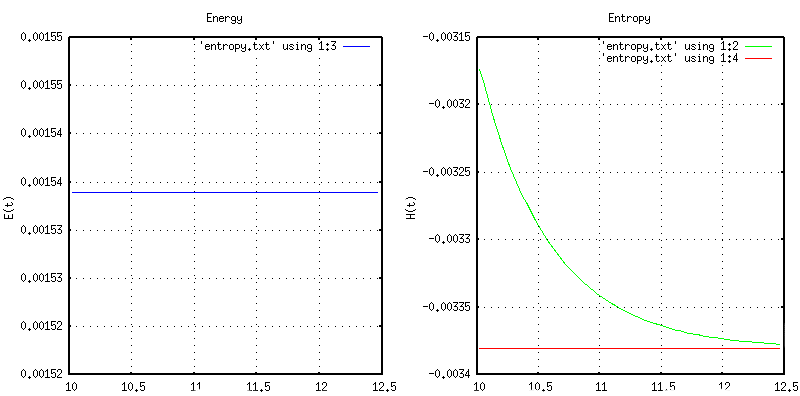
\includegraphics[scale=0.5]{entropy_plot_limit}

Our results here verify that the distribution converges to an equilibrium
state which factorizes:

\[
\lim\limits _{t\rightarrow\infty}f(A,B,t)=\frac{1}{\rho}\intop f(A,B')f(A',B)dA'dB'
\]


And after integrating out A' and B', we have:

\[
\lim\limits _{t\rightarrow\infty}f(A,B,t)=f(A)f(B)
\]


Which is exactly the requirement required by statistical mechanics
proper for a probability density to equilibrate. The red line represents
the entropy limit to which the entropy of the system will converge
to at $t=\infty$. We are using sloppy language here because H is
not really entropy, so the ``entropy limit'' is really the ``H
limit'' but disregarding the minus sign, these are really the same
quantities. It is calculated in the following way:

\[
f(A)=\int\frac{f(\mathbf{A},\mathbf{B})}{\rho}d\mathbf{B}
\]


\[
f(B)=\int\frac{f(\mathbf{A},\mathbf{B})}{\rho}d\mathbf{A}
\]


\[
\mathcal{H}_{lim}=\int\rho f(\mathbf{A})f(\mathbf{B})ln(\rho f(\mathbf{A})f(\mathbf{B}))
\]


And in terms of the Lebedev Quadrature:

\[
f(A)=\sum_{B}^{n}\frac{f(A,B)w_{B}}{\rho}
\]


\[
f(B)=\sum_{A}^{n}\frac{f(A,B)w_{A}}{\rho}
\]


\[
\mathcal{H}_{lim}=\sum_{A}^{n}\sum_{B}^{n}f(A)f(B)\, ln(\rho f(A)f(B))\, w_{A}w_{B}
\]



\subsection{Energy-Momentum Tensor}

We can calculate the energy-momentum tensor by calculating the average
x, y, and z values. This will allow us to calculate the pressure and
the equation of state parameter p.

\[
p=\rho w
\]


We know how to calculate $\rho$, but the equation of state parameter
is found through averaging over A and B, grabbing the Cartesian coordinates,
then building a 3x3 matrix from the resulting quantities. 

\[
<A>=\int Af(A,B)dB
\]


\[
<B>=\int Bf(A,B)dA
\]


Then the energy-momentum tensor is:

\[
T_{ij}=\frac{<A_{i}><B_{j}>}{\rho}
\]


Thus,

\[
w=\frac{Tr\left(F_{ij}\right)}{3\rho}
\]



\section{Adding the Gravitational Term}


\subsection{Introduction}

In the previous section we determined that collisions between string
segments could be modeled using (4). However, we made some assumptions
in neglecting the other two terms in (1). In fact, ignoring the spatial
and gravitational terms, the transport equation is valid in Minkowski
space. But for a non trivial metric, such as one that includes expansion,
we must add a new term which accounts for the effects. We'll still
be ignoring the spatial term for now. 

The actual terms for $\left(\frac{df}{dt}\right)_{gravitational}$
come from the left hand side of (2). Namely, the stuff with the Hubble
parameter $\mathcal{H}$ attached:

\begin{equation}
\left(\frac{df}{dt}\right)_{gravitational}=\mathcal{H}\left(\partial_{A}+\partial_{B}-(1+A\cdot B)-4(A\cdot B)\right)f(A,B)
\end{equation}


The operators $\partial_{A}$ and $\partial_{B}$ can be reduced to
theta derivatives:

\[
\partial_{A}=sin(\theta_{B})\frac{\partial}{\partial\theta_{B}}
\]


\[
\partial_{B}=sin(\theta_{A})\frac{\partial}{\partial\theta_{A}}
\]


We can access the components of each Point object, so we can actually
represent these operators as something workable now:

\begin{equation}
\partial_{A}=-\sum_{i=1}^{3}B_{i}sin(\theta_{i})\frac{\partial}{\partial\theta_{i}}
\end{equation}


\begin{equation}
\partial_{B}=-\sum_{i=1}^{3}A_{i}sin(\theta_{i})\frac{\partial}{\partial\theta_{i}}
\end{equation}


Here, i ranges over the Cartesian components of the Point A and B
just like before, but the derivative term $\frac{d}{d\theta_{i}}$
is something new. These operators take the theta derivative in the
$i$ direction on the sphere. So we'd like a way to easily take derivatives
of f(A,B) along x, y, and z with respect to theta. Then we act these
operators on f(A,B) at every time step, and add this effect in as
we update the distribution function. The first step is to create a
new array that holds the values of $\left(\frac{df}{dt}\right)_{grav}$.
So in the end, equation (21) is another 2-d array:

\begin{algorithm}[!h]
\begin{algor}
\item [{for}] \ensuremath{(A=0;\, A<N;\, A++)}


\begin{algor}
\item [{for}] $(B=0;\: B<N;\: B++)$

\begin{algor}
\item [{{*}}] $df_{g}[A][B]=\mathcal{H\,}(\,\partial_{A}[A][B]+\partial_{B}[A][B]-1-5(Point[A]\circ Point[B])\,)\, f[A][B]\Delta t$ 
\end{algor}
\item [{endfor}]~
\end{algor}
\item [{endfor}]~
\end{algor}
\caption{Calculate the gravitational term $\left(df(A,B)\right)_{grav}$}
\end{algorithm}


And then we update the distribution function f(A,B) like in Algorithm
8:

\begin{algorithm}[!h]
\begin{algor}
\item [{for}] \ensuremath{(A=0;\, A<N;\, A++)}


\begin{algor}
\item [{for}] $(B=0;\: B<N;\: B++)$

\begin{algor}
\item [{{*}}] $f[A][B]=f[A][B]+df[A][B]+df_{g}[A][B]$ 
\end{algor}
\item [{endfor}]~
\end{algor}
\item [{endfor}]~
\end{algor}
\caption{Update the distribution with the gravitational term}
\end{algorithm}


But how do we calculate the terms that go into $\left(\frac{df}{dt}\right)_{grav}$?
We'll ignore the derivative terms for now (we'll deal with them in
the next section). We know how to take the dot product between the
two point objects \textbf{A} and \textbf{B}. Likewise, the Hubble
parameter $\mathcal{H}$ is a function of of the time $\tau$, and
is simple to calculate. This is the term that adds the expansion due
to the metric. In particular, we'll be dealing with the Friedmann
metric in conformally flat space-time:

\medskip{}


\[
ds^{2}=a^{2}(t)(t^{2}-x^{2}-y^{2}-z^{2})
\]


\[
\mathcal{H}=\left(\frac{\dot{a}}{a}\right)
\]


\[
a(t)\propto t^{\frac{2}{n}}
\]


\begin{equation}
\rho\propto a^{-n}\propto t^{-\frac{2}{n}}
\end{equation}


\medskip{}


What we are interested in doing is having a function that accounts
for expansion as a function of time. In Cosmology, this is the role
that the Hubble parameter plays. We can find an expression for it
by using the fact that the scale factor a($\tau$) is expressed as
a function of time, and likewise for its derivative:

\medskip{}


$\dot{a}(t)\propto\left(\frac{2}{n}\right)t^{(\frac{2}{n}-1)}$

$\mathcal{H}=\left(\frac{\dot{a}}{a}\right)\propto\frac{(\frac{2}{n})t^{(\frac{2}{n}-1)}}{t^{\left(\frac{2}{n}\right)}}\propto\frac{2}{nt}$
where n is an integer which takes on values of 2,3, and 4. 

\medskip{}


These n-values correspond to different eras in the expansion rate
of the universe. When the universe was too hot for normal matter to
form, n=4. This is referred to as a radiation dominated expansion
rate. The Hubble parameter is $\mathcal{H}=\frac{1}{2t}$ for this
era. Likewise, the matter dominated era refers to later times, and
$\mathcal{H}=\frac{2}{3t}$. The quantity which we can probe comes
from (12). It implies that when we include expansion in either of
these two eras, we should find that the energy density falls off as
$-\frac{2}{3}$ for matter dominated, and $-\frac{1}{2}$ for radiation.
If we look at a log-log plot of energy density vs time, we will find
that the slope of that line should match the predictions for the rate
(either $-\frac{2}{3}$ $or-\frac{1}{2}$ ). This will be a powerful
test to determine if the gravitational term is working. However, there
is a caveat. This prediction for the energy density to fall off at
a rate of $-\frac{2}{n}$ is only valid for particular initial conditions. 

Recall from the introduction that we defined two quantities, u and
v. These were unit vectors that describe the longitudinal and transverse
velocities along strings. The predicted numerical values of the energy
density decay's power are only valid in the case where $<v^{2}>=\frac{1}{2}$.
Using the VMF distribution, we can choose initial conditions such
that we have large peaks that point in the same direction on both
the A and B spheres as discussed in section 1.3. By setting up the
initial conditions correctly (a=b), we can set to start out near $<v^{2}>=\frac{1}{2}$
and watch as the system evolves to see how the energy density falls
off. 

So we need a way of calculating \textbf{v}, such that we can check
the decay rate of the energy density. Fortunately, this is easy. To
calculate the expectation value of a quantity using a probability
density, we simply integrate over the density function while multiplying
by the quantity which we want averaged. Since u and v are just functions
of A and B, we have:

\medskip{}


\[
<v^{2}>=\int\frac{v^{2}f(\mathbf{A},\mathbf{B})d\mathbf{A}d\mathbf{B}}{\rho}
\]


\medskip{}


where $\mathbf{v}=\frac{\mathbf{A}+\mathbf{B}}{2}$

\medskip{}


Then, we can also define $<v>^{2}$, which we need $<\mathbf{v}>$
to calculate:

\[
<\mathbf{v}>=\intop\frac{\mathbf{v}\, f(\mathbf{A},\mathbf{B})d\mathbf{A}d\mathbf{B}}{\rho}
\]


Then, 
\[
<v>^{2}=<\mathbf{v}>\circ<\mathbf{v}>
\]


And likewise for \textbf{u}. The pseudo-code is what you'd expect:

\begin{algorithm}[!h]
\begin{algor}
\item [{for}] \ensuremath{(A=0;\, A<N;\, A++)}


\begin{algor}
\item [{for}] $(B=0;\: B<N;\: B++)$

\begin{algor}
\item [{{*}}] $v=v+(\frac{Point[A]+Point[B]}{2})\, f[A][B]\, Point[A].GetWeight()\, Point[B].GetWeight()$\{recursive
definition of $<v>$\}
\item [{{*}}] $v^{2}=v^{2}+(\frac{Point[A]+Point[B]}{2})\circ(\frac{Point[A]+Point[B]}{2})\, f[A][B]\, Point[A].GetWeight()\, Point[B].GetWeight()$\{recursive
definition of $<v^{2}>$\}
\end{algor}
\item [{endfor}]~
\end{algor}
\item [{endfor}]~
\end{algor}
\caption{Update the distribution with the gravitational term}
\end{algorithm}


Here $<\mathbf{v}>$ is a vector, while $<v^{2}>$ is a scalar. Then
$<\mathbf{v}>^{2}$ is found by dotting $<\mathbf{v}>$ with itself,
which also ends up being scalar.

We can do the same for the quantities $<\mathbf{u}>^{2}$ and $<u^{2}>$.
Outputting these quantities will help us later on to determine if
the gravitational terms are being calculated correctly. Since \textbf{v}
and \textbf{u} are vector fields, we can compute field lines by running
the simulation with different initial conditions, and then plot $<v>^{2}$
and $<u>^{2}$ as the system equilibrates:

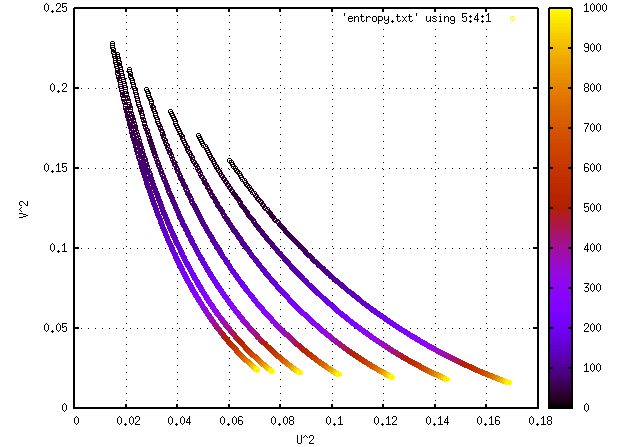
\includegraphics[scale=0.5]{fieldlines}

The above plots were made by running through the simulation for 1000
time steps (color map), and then changing the mean direction as determined
by the VMF distribution function given in section 1.3. We varied the
mean direction of the initial conditions (i.e. where the peak of the
distribution was highest) by changing the constant vectors \textbf{a}
and \textbf{b} for each run. 

Now we are ready to move on to calculating the derivative terms.


\subsection{Integral Transform and Kernels}

We now want to numerically compute the derivative terms in (11). There
are many ways to take derivatives numerically, but because of our
Lebedev points, the method we'll be using involves Spherical Harmonics.
The way we calculate derivatives on the sphere using spherical harmonics
is rooted in an integral transform. From this, we find an operator
known as a ``Kernel''. 

To find the derivative of $f(\theta,\phi)$, we must use a kernel,
which is obtained through the integral transform. The general integral
transform is defined as:

$(Tf)(u)=\int\limits _{x_{1}}^{x_{2}}K(x,u)\, f(x)\, dt$ 

Where K is the kernel of the function. The kernel is then an operator
by which we multiply f(x) in order to obtain the transform. In our
case, the input of the transform will be $f(\theta,\phi)$, and the
output is another function $Tf=f(\theta',\phi')$. The Lebedev points
serve as a way to guarantee that this condition is met for all points
on the sphere over which we integrate (recall that the Lebedev points
have octahedral symmetry). 

For a polynomial on the sphere, $f(\theta,\phi)=P_{m}^{l}(\cos(\theta))$$e{}^{im\phi}C_{m}^{l}$;
we can calculate the derivative using spherical harmonics and the
integral transform. The general expression for a spherical harmonic
is:

\medskip{}


$Y_{m}^{l}=\sqrt{\frac{2l+1}{4\pi}\frac{(l-m)!}{(l+m)!}}P_{m}^{l}(\cos(\theta))e{}^{im\phi}$

\medskip{}


Using this method, we can construct the derivative of $f(\theta,\phi)$
using the kernel from the transform. 

\medskip{}


$\frac{d}{d\theta}f(\theta',\phi')={\displaystyle \sum_{l=0}^{\infty}{\displaystyle \sum_{m=-l}^{l}}}C_{m}^{l}\,\frac{d}{d\theta}Y_{m}^{l}(\theta',\phi')$

\medskip{}


where

\medskip{}


$C_{m}^{l}=\int\, Y_{m}^{l}(\theta,\phi)*f(\theta,\phi)\, d\Omega$

\medskip{}


Thus,

\medskip{}


$\frac{d}{d\theta}f(\theta',\phi')={\displaystyle \sum_{l=0}^{\infty}{\displaystyle \sum_{m=-l}^{l}}}\int\, Y_{m}^{l}*f(\theta,\phi)\, d\Omega_{m}^{l}\,\frac{d}{d\theta}Y_{m}^{l}(\theta',\phi')$

\medskip{}


Now, we can rearrange the integral into a more convenient form:

\medskip{}


\begin{equation}
\frac{d}{d\theta}f(\theta',\phi')=\int\, f(\theta,\phi)\,{\displaystyle \sum_{l=0}^{\infty}{\displaystyle \sum_{m=-l}^{l}}}Y_{m}^{l}(\theta,\phi)*\frac{d}{d\theta}Y_{m}^{l}(\theta',\phi')\, d\Omega
\end{equation}


\medskip{}


The summation within the integral is then the Kernel of this transform.
Because it is independent of $f(\theta,\phi)$, can calculate it separately.
This allows us to save a lot of computation time because we can calculate
the kernel once, save it, and then iterate through the file to calculate
the derivative. Thus,

\medskip{}


\[
K(\theta',\phi',\theta,\phi)={\displaystyle \sum_{l=0}^{\infty}{\displaystyle \sum_{m=-l}^{l}}}Y_{m}^{l}(\theta,\phi)*\frac{d}{d\theta}Y_{m}^{l}(\theta',\phi')
\]


\medskip{}


where

\medskip{}


$\frac{d}{d\theta}Y_{m}^{l}(\theta',\phi')=m\, cot(\theta')\, Y_{m}^{l}\,+\sqrt{(l-m)(l+m+1}e^{-i\phi}Y_{m+1}^{l}$

\medskip{}


Then, when we want the derivative we simply integrate:

\medskip{}


\begin{equation}
\frac{d}{d\theta}f(\theta',\phi')=\int\, f(\theta,\phi)\, K\, d\Omega
\end{equation}


\medskip{}


Likewise, if we replace $\frac{d}{d\theta}Y_{m}^{l}(\theta',\phi')$
with $Y_{m}^{l}(\theta',\phi')$ in the kernel, we can use the same
method to reconstruct the function as well. This has served as useful
verification tool to show our method is working correctly because
of the complicated functions required to build the kernel. For instance
if we build two separate kernel files, one for the derivative and
one for $\frac{d}{d\theta}Y_{m}^{l}(\theta',\phi')$ and one for $Y_{m}^{l}(\theta',\phi')$,
we can test whether or not the method of building the kernel file
is wrong, or if there is something in particular about the derivative
of the spherical harmonic which is causing the kernel to reproduce
the derivatives of known functions incorrectly.


\subsection{Building the Kernel file}

The code referenced in {[}6{]} is written in C++ and uses Boost libraries
to calculate Spherical Harmonics. So depending on your language of
choice, the following method may or may not work. Calculating the
Spherical Harmonics manually is not so difficult, but special attention
needs to be given to points at the poles on the sphere. As usual,
m ranges from -l to l. The meaning integer l however corresponds to
the order of accuracy to which we choose to estimate functions on
the sphere. You will notice in the code given in {[}6{]} that l is
defined from the Lebedev points. When you run the code, the first
step you take will be to define the precision with which you'd like
to run the model. This precision refers to the rule you are using
to define your Lebedev points, and higher l requires more points to
estimate, which in turn requires longer computations because the loop
size increases. It's best to show you the algorithm for building the
Kernel file and then explain what it is doing. Recall that the kernel
function looks like:

\begin{equation}
K(\theta',\phi',\theta,\phi)={\displaystyle \sum_{l=0}^{\infty}{\displaystyle \sum_{m=-l}^{l}}}Y_{m}^{l}(\theta,\phi)*\frac{d}{d\theta}Y_{m}^{l}(\theta',\phi')
\end{equation}


\begin{equation}
\frac{d}{d\theta}Y_{m}^{l}(\theta',\phi')=m\, cot(\theta')\, Y_{m}^{l}\,+\sqrt{(l-m)(l+m+1}e^{-i\phi}Y_{m+1}^{l}
\end{equation}


This tells us that we need a four dimensional function that sums over
all m for a given value of l. Using the Lebedev points, each function
of $\theta,\phi$ can be represented in one loop. Let's call our two
spherical harmonic functions $Y$ and $Y'$ respectively. The $Y'$
will be iterated over i in the outer loop as $Y'(\theta',\phi')$
and $\frac{d}{d\theta}Y'(\theta',\phi')$, and the inner loop will
iterate over $Y(\theta,\phi)$. The derivative of $Y$ will be referred
to as $dY'$. Then we have the following loop to produce the Kernel
file:

\medskip{}


\begin{algorithm}[!h]
\begin{algor}
\item [{Require:}]~
\end{algor}
{*} $GenerateKernel(N,L)$ \{function call where L is the order of
the polynomial, and N is the number of points\}

{*} $array\; dkernel[n][n]$ \{arrays to store kernel values\}

{*} $array\; fkernel[n][n]$ 

{*} $complex\; Y,\, Y',\, dY'$ \{complex double variables for use
with the spherical harmonics\}
\begin{algor}
\item [{for}] \ensuremath{(A=0;\, A<N;\, A++)}


\begin{algor}
\item [{for}] $(B=0;\: B<N;\: B++)$

\begin{algor}
\item [{for}] \ensuremath{(A=0;\, A<N;\, A++)}


\begin{algor}
\item [{for}] $(B=0;\: B<N;\: B++)$
\item [{{*}}] $Y'=SphericalHarmonic(m,l,Point[i].GetTheta(),Point[j].GetPhi())$
\item [{{*}}] $Y=SphericalHarmonic(m,l,Point[j].GetTheta(),Point[j].GetPhi())$

\begin{algor}
\item [{if}] $(m+1\leq l\;\mathbf{and\;}Point[i].GetTheta()\neq0)$\{prevent
division by zero\}
\item [{do}]~
\item [{{*}}] $dY'=m\, cot(Point[i].GetTheta())\, Y'+\sqrt{(l-m)(l+m+1)}e^{-\mathbf{i}\, Point[i].GetPhi()}SphericalHarmonic(m+1,l,Point[i].GetTheta(),Point[i].GetPhi())$
\item [{endif}] \{\textbf{i} in boldface is $\sqrt{-1}$\}
\item [{{*}}] $fkern[i][j]=fkern[i][j]+Y^{*}Y'$ \{where {*} is the complex
conjugate\}
\item [{{*}}] $dkern[i][j]=dkern[i][j]+Y^{*}dY'$
\end{algor}
\item [{endfor}]~
\end{algor}
\item [{endfor}]~
\end{algor}
\item [{endfor}]~
\end{algor}
\item [{endfor}]~
\end{algor}
\caption{Generate the Kernel file}
\end{algorithm}


\begin{algorithm}[!h]
\begin{algor}
\item [{Require:}]~
\end{algor}
{*}$makefile("DerivativeKernel.dat")\; dfile$ \{a data file for derivative
kernel\}

{*}$makefile(\lyxmathsym{\textquotedblleft}FunctionKernel.txt\lyxmathsym{\textquotedblright})\: ffile$
\{a data file for function kernel\}
\begin{algor}
\item [{for}] \ensuremath{(i=0;\, i<N;\, i++)}


\begin{algor}
\item [{for}] $(j=0;\: j<N;\: j++)$

\begin{algor}
\item [{{*}}] $dfile(dkern[i][j]\, Point[j].GetWeight())$ 
\item [{{*}}] $ffile(fkern[i][j]\, Point[j].GetWeight())$\{fill the data
file with tab-delineated values, multiply by the weights\}
\end{algor}
\item [{endfor}]~
\end{algor}
\item [{endfor}]~
\end{algor}
\caption{Update the distribution with the gravitational term}
\end{algorithm}


Let's unpack this. First, we declare some files in which to store
the kernels. We want a kernel to reconstruct functions, and one to
reconstruct derivatives. The one used to reconstruct functions is
not necessary for the model, but it will allow you to trouble shoot
any general problems with the construction of the kernels. Depending
on how you calculate the spherical harmonics, you will likely end
up with complex numbers which you can deal with as you choose. For
a good introduction to coding Spherical Harmonics, see reference {[}8{]}.
The code in {[}6{]} allows for complex math and the Boost libraries
for C++ include a function for calculating spherical harmonics. However,
the theta derivative of a spherical harmonic is not usually included,
and one must use an explicit formula like the one given by (18). Notice
the if condition in calculating $dY'$. We exclude the pole where
$\theta$ is zero since the cotangent function blows up there. We've
also been careful to exclude the case where we plug m+1>l into the
SphericalHarmonic() function because some libraries will not deal
with this exception. The function should spit back zero, but if not,
deal with the case like above and $dY'$ will always be zero at the
m+1>l case. 

We then sum over the l and m values as we load them into the kernel
arrays. Finally, save the arrays to file as they are, but multiply
by the weights so we don't have to map those as well. The weights
can be safely absorbed into the Kernel. Now we can save Kernels for
arbitrary numbers of Lebedev points and orders. You can produce some
very big kernels and use these to quickly do take derivative at high
order. This will allow us to compute the gravitational terms quickly
in our main code. In C++, and using the Boost libraries as in {[}6{]},
we can speed up the algorithm by filling an array with the Y value
for each l and m. This reduces the heavy dependence on l from the
inner-most loop, and also takes some pressure off the efficiency of
the Spherical Harmonics algorithm contained within the Boost libraries. 


\subsection{Reconstruction of functions using a Kernel}

We now have a way of estimating derivatives using the Kernel. The
next step will be testing some functions with known derivatives and
seeing how they reconstruct. During the tests, we'll be varying l
and the number of points as we generate new kernels to explore how
well (or how poorly) the functions and their derivatives reconstruct
at low and high orders. For the file used in the distribution simulation,
we will use a 2-dimensional array to find the derivative at each A,
and B. The order of l need not be fixed for the derivative terms in
the distribution function if we build the kernel to allow for access
to each l. Of course this increases the size of your Kernel because
the arrays used to store the kernels now include an extra dimension
for l. The downfall of this approach is it increases the size of the
file and the time it takes to put the new kernel into memory. But
you should only need to do this once. The code in {[}6{]} is set to
be calculated at fixed l. However, it can be easily modified by increasing
the array size to allow for an extra dimension for l. It's important
to understand how the order is related to number of points and the
quality of the reconstructions we can obtain using this method. If
we choose l wisely, we can build a kernel for a particular l value
and certain number of points that runs in a timely way when we start
doing the numerical approximation. And the benefit of using the kernel
in this way is that we only need to construct it one time, and then
we're free to use that kernel file in trial runs later on. 

The nature of the Lebedev points requires that the order (l) not exceed
the precision of a given set of weights and points. For instance,
the precision of the 5810-point set is 131, thus l must be less than
or equal to 131, or else even well-behaved functions (or derivatives)
will not reconstruct at all. Choosing $l<precision$ allows for successful
reconstruction of well-behaved functions and their corresponding derivatives.
However, for not-so-well-behaved functions, (i.e. functions with discontinuities
or noise) high frequency oscillations occur throughout the reconstructed
function, and it gets worse as l approaches the precision value for
the set of points used.

The correlation between the number of Lebedev points and the order
to which we solve spherical harmonics is analogous to the Nyquist
Frequency, in which we must have some minimum number of sample points
(the Lebedev points) in order to successfully reconstruct a function
over which we're sampling at some frequency (the order l in our case). 

\medskip{}


First, load the kernel into a 2-d array. You'll need to be able to
integrate over it using the quadrature method from (6), as well as
locate particular elements, so an object that holds the array and
has a function like GetKernelElement(i,j) would be preferred. In the
code referenced in {[}6{]}, the object that holds the Kernel in memory
is referred to as Mapper. It contains a function for retrieving a
particular kernel element from the data file saved as in Algorithm
13. Then, we can setup the equation (15) from the previous section.
We'll also need an array that stores values from a function of the
Lebedev points. To start, in spherical coordinates:

\medskip{}


$x=sin(\theta)cos(\phi)$

$y=sin(\theta)sin(\phi)$

$z=cos(\theta)$

\medskip{}


$\frac{d}{d\theta}x=cos(\theta)cos(\phi)$

\medskip{}


Combinations of these functions are Spherical Harmonics, so if your
Kernel is working, derivatives of them should reconstruct exactly
if the order l is chosen correctly. Let's first differentiate x using
the kernel. Evaluate $sin(\theta)cos(\phi)$ using the Lebedev points
and load the results into an array, $x[]$. Well you are at it, load
the derivative of that function into another array, $dx[]$ as well
so you can compare the results in the next step. Then we'll take that
array and set it up like in (15). We've labeled the object which contains
the Kernels and element retrieval functions as ``Mapper'', and the
functions that return the Kernel elements as GetFKernel(i,j) and GetDKernel(i,j)
for the function kernel and derivative kernel, respectively. Now we
just integrate in the usual way, but leaving out the weights since
we already absorbed them into the kernel file's elements (Algorithm
14):

\begin{algorithm}[!h]
\begin{algor}
\item [{for}] \ensuremath{(i=0;\, i<N;\, i++)}


\begin{algor}
\item [{for}] $(j=0;\: j<N;\: j++)$

\begin{algor}
\item [{{*}}] $\partial_{f}[i]=\partial_{f}[i]+x[j]\, Mapper.GetDKernel(i,j)$
\item [{{*}}] $f[i]\,=\, f[i]+x[j]\, Mapper.GetFKernel(i,j)$
\end{algor}
\item [{endfor}]~
\end{algor}
\item [{endfor}]~
\end{algor}
\caption{Evaluate a function x{[}{]} with the kernels. f{[}{]} is a reconstructed
version of the function, and $\partial_{f}[]$ is the derivative of
the function using the kernel files we constructed in Algorithm 13
\& 14.}
\end{algorithm}


Now you have a reconstructed derivative $\partial_{f}$ and a reconstructed
function $f$ using your two kernels developed in the last section.
You should see numerical values that match every element in dx{[}{]}
and x{[}{]} respectively. If f{[}{]} reconstructs correctly but $\partial_{f}[]$
does not, your method of creating the kernel is functioning properly,
but there is likely a problem with the formula used for the theta
derivative of the spherical harmonic. With 110 points and an order
l=12, we have:

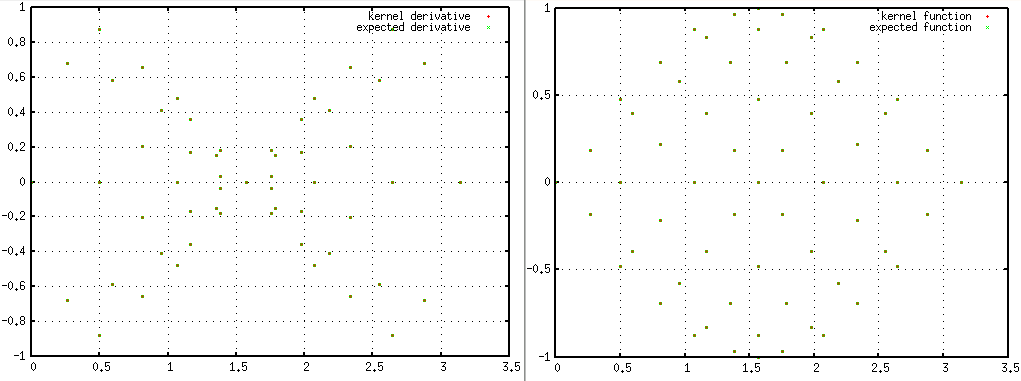
\includegraphics[scale=0.4]{l16_110}

But what happens if we choose l=17 (the limit for 110 points)? The
estimate is no longer exact:

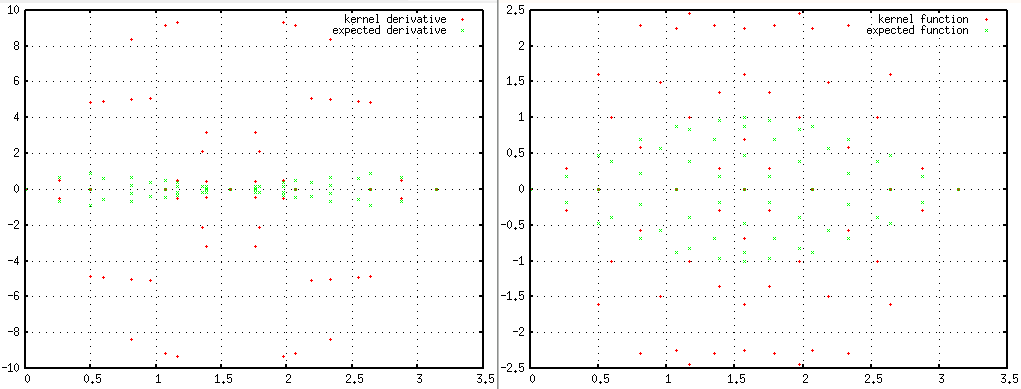
\includegraphics[scale=0.4]{l17_110}

So the order at which we build the kernel files will greatly affect
how accurate the derivative approximations are. We must choose l<precision
of the Lebedev points or the method does not work.


\subsection{Rotation using the Kernel}

Recall that equations (12) and (13) require our operators for $\partial_{A}$
and $\partial_{B}$ to contain derivatives of the sphere in the x,
y and z direction. By rotating the sphere by $\frac{\pi}{2}$ in both
theta and phi, we can find the derivative with respect to theta along
any axis using the same kernel we calculated above. But we need a
method for rotating our Lebedev points to do so. Assuming the first
derivative calculated was along the z-axis, we can find both the x-axis
and y-axis derivatives by performing a rotation of the points and
then integrating over the kernel as was shown in the last section. 

The rotation is performed by converting the spherical coordinates
to Cartesian, and swapping values such that the symmetry of the Lebedev
points is maintained. Because the Lebedev points and their corresponding
weights are produced with Octahedral symmetry, we can rotate the points
in any way that would also preserve the symmetry of a cube. That is,
if we rotate z by $\frac{\pi}{2}$ in the theta direction (holding
phi at zero), our new point is at -y. As an example, let's rotate
points about y ($\theta_{y}$):

\medskip{}


$x\rightarrow-z$

$y\rightarrow y$

$z\rightarrow x$

\medskip{}


And likewise, about x ($\theta_{x}$):

\medskip{}


$x\rightarrow x$

$y\rightarrow z$

$z\rightarrow-y$

\medskip{}


Recall in Section 1 that we said we'd need our Point object to have
the capability to convert between Spherical and Cartesian coordinates.
This will be an important function now. What we'd like to do is have
a function that takes in theta and phi components from the Lebedev
files, then converts those components to Cartesian coordinates, and
then allows us to access them through our old function GetX(), GetY(),
and GetZ(). Then, we can do the following to create a list of rotated
points. For the rotation about x, y and z, let's make arrays of point
objects called ListX, ListY, and ListZ, and the original point object,
Point. Then we can do the following:

\begin{algorithm}[!h]
\begin{algor}
\item [{for}] $(i=0;\: i<N;\: i++)$ 

\begin{algor}
\item [{{*}}] $ListX[i].SetCartesian(Point[i].GetX(),\, Point[i].GetZ(),\,-Point[i].GetY())$\{rotation
about X\}
\item [{{*}}] $ListY[i].SetCartesian(Point[i].GetZ(),\, Point[i].GetY(),\,-Point[i].GetX())$\{rotation
about Y\}
\item [{{*}}] $ListZ[i].SetCartesian(Point[i].GetX(),\, Point[i].GetY(),\, Point[i].GetZ())$
\{this list is redundant\}
\end{algor}
\item [{endfor}]~
\end{algor}
\caption{Setup rotated lists of Lebedev points}
\end{algorithm}


With these three lists, we are set to evaluate the derivative along
the X, Y, or Z axis of the sphere. But there is a catch. Our kernel
was produced using the original Lebedev points, so calculating the
derivative along another axis other than the original is not possible
unless we can find the points in the kernel that correspond to the
rotation. Of course, all of the points are present, just out of order.
The next step involves a quick search algorithm to find the rotated
points and build and iterator to find the Kernel. This will allow
us to take derivatives with respect to theta along x, y, and z for
(12) and (13). 

Using a simple search algorithm we can find the rotated points within
just one kernel file, and then save the location of the points to
an iterator object and use that to evaluate the integral at the correct
Lebedev points when we evaluate the derivative. This saves us a lot
of memory because we only need one kernel. The idea is to apply the
rotation to the iterators and use those to produce rotated kernel
values that correspond to the rotated Lebedev points and weights.
The algorithm goes as follows:

\begin{algorithm}[!h]
\begin{algor}
\item [{for}] $(i=0;\: i<N;\: i++)$ 

\begin{algor}
\item [{for}] $(j=0;\: j<N;\: j++)$ 

\begin{algor}
\item [{if}] $Point[i]=ListX[j]$
\item [{{*}}] $map[i]=j$
\item [{endif}]~
\end{algor}
\item [{endfor}]~
\end{algor}
\item [{endfor}]~
\end{algor}
\caption{Create map to rotated points}
\end{algorithm}


Now, we simply use the map array to find the rotated points in the
kernel file. The kernel 

\begin{algorithm}[!h]
\begin{algor}
\item [{for}] $(i=0;\: i<N;\: i++)$ 

\begin{algor}
\item [{for}] $(j=0;\: j<N;\: j++)$ 

\begin{algor}
\item [{{*}}] $kernel_{map}[i][j]=kernel_{original}[\, map[i]\,][\, map[j]\,]$
\end{algor}
\item [{endfor}]~
\end{algor}
\item [{endfor}]~
\end{algor}
\caption{Use map as iterator to find rotated points in kernel file}
\end{algorithm}


The object we called ``Mapper'' in the previous section was an object
which contained functions like GetDkernel() and GetFKernel(). These
functions should retrieve the elements of the $kernel_{map}[][]$
array which contains the rotated points. 

The next step would be to define ListX{[}{]} a little more abstractly,
such that when the function that calculates the gravitational terms
needs a particular rotation, ListX{[}{]} changes to ListY{[}{]} or
ListZ{[}{]}. The code in {[}6{]} does this in an object oriented way,
by creating separate objects that correspond to each rotated kernel,
and then uses these arrays to calculate the derivatives in the x,
y, and z directions, as will be seen in the next section.

The iterator object, map{[}{]} just holds the index value of the point
that was found. Then when we want to build the rotated map of the
kernel, we simply fill the map array up with the values from the original
file that correspond to the rotated index. Now, with this function
we can specify the axis of rotation we'd like to have, and retrieve
the associated kernel. Example plots of the function $f(\theta,\phi)=cos(\theta)cos(\phi)$
plotted using the above technique to determine the rotation about
x,y, and z (in that order) using 1200 points and l=20:

\begin{tabular}{|c|c|c|}
\hline 
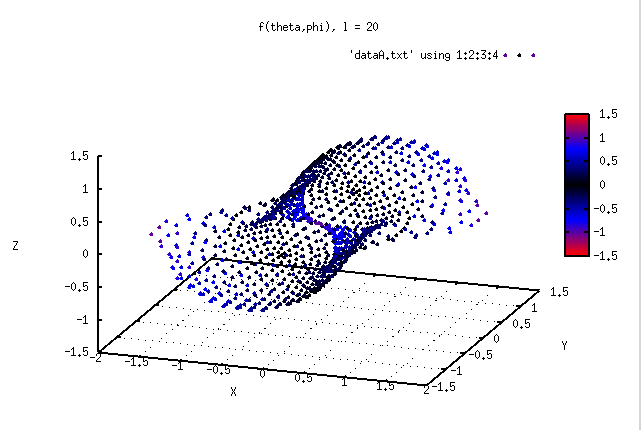
\includegraphics[scale=0.2]{X} & 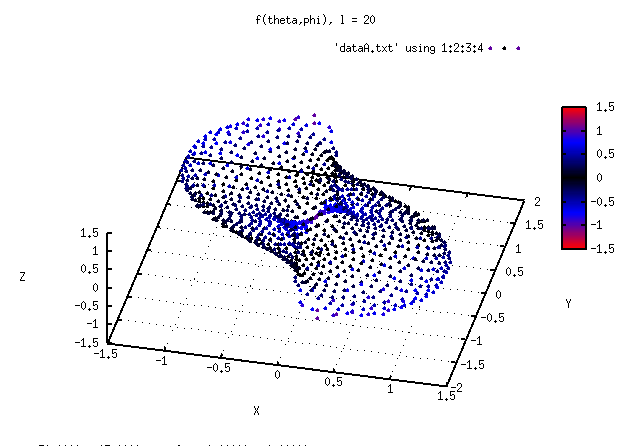
\includegraphics[scale=0.2]{Y} & 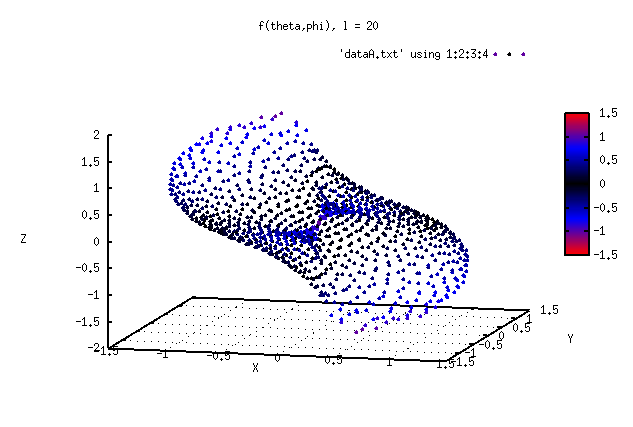
\includegraphics[scale=0.2]{Z}\tabularnewline
\hline 
\end{tabular}

In summary, we have a function that gives us a kernel file which acts
as a derivative operator when integrated over. We found that we could
take the derivative along different axis of the sphere by embedding
it in $\mathbb{R}^{3}$ and performing rotations on the kernel file
such that the theta derivative operator (the kernel) would be taken
in different directions corresponding to rotations about the Cartesian
coordinates. Now we can take derivatives of functions of A and B,
which is exactly the distribution function f(A,B).

\medskip{}



\subsection{Calculating the Gravitational Term}

Now we will put everything done in the last few sections together
to calculate $\left(\frac{df}{dt}\right)_{gravitational}$. We now
know how to take derivatives using the Kernel. We setup an object
which contains the rules for rotating the kernel. This object is just
like a Point object in that it contains functions like GetTheta(),
and GetPhi(), but the difference is that when you instantiate it,
it calls GenerateKernel(), and in so doing prepares an accessor array
that contains the rotated Lebedev points as well as as the Kernel
itself. We make three of these objects using three different maps,
one for each rotation, called RotatedAboutX, RotatedAboutY, and RotatedAboutZ.
Each contains a map of the original kernel. Then, we take the derivatives
just like we've done in the previous section. Recalling that the weights
have been absorbed into the kernel, then our algorithm for $\partial_{A}$
from (eq. 22) looks like:

\[
\partial_{A}=-\sum_{i=1}^{3}B_{i}sin(\theta_{i})\frac{\partial}{\partial\theta_{i}}
\]


\begin{algorithm}[!h]
\begin{algor}
\item [{for}] $(B=0;\: B<N;\: B++)$ 

\begin{algor}
\item [{for}] $(k=0;\: k<N;\: k++)$ 

\begin{algor}
\item [{{*}}] $dA_{x}[B]=dA_{x}[B]+f[k][B]\, RotatedAboutX.GetDKernel(B,k)$
\item [{{*}}] $dA_{y}[B]=dA_{y}[B]+f[k][B]\, RotatedAboutY.GetDKernel(B,k)$
\item [{{*}}] $dA_{z}[B]=dA_{z}[B]+f[k][B]\, RotatedAboutZ.GetDKernel(B,k)$
\end{algor}
\item [{endfor}]~
\end{algor}
\item [{endfor}]~
\item [{for}] $(A=0;\: A<N;\: A++)$ 

\begin{algor}
\item [{for}] $(B=0;\: B<N;\: B++)$ 

\begin{algor}
\item [{{*}}] $\partial_{A}[A][B]=$
\item [{{*}}] $-Point[B].GetX()\, sin(RotatedAboutX.GetTheta(A))\, dA_{x}[A]$
\item [{{*}}] $-Point[B].GetY()\, sin(RotatedAboutY.GetTheta(A))\, dA_{y}[A]$
\item [{{*}}] $-Point[B].GetZ()\, sin(RotatedAboutZ.GetTheta(A))\, dA_{z}[A]$
\end{algor}
\item [{endfor}]~
\end{algor}
\item [{endfor}]~
\end{algor}
\caption{Calculate $\partial_{A}$}
\end{algorithm}


And likewise for $\partial_{B}$, from (eq. 23) we have:

\[
\partial_{B}=-\sum_{i=1}^{3}A_{i}sin(\theta_{i})\frac{\partial}{\partial\theta_{i}}
\]


\begin{algorithm}[!h]
\begin{algor}
\item [{for}] $(A=0;\: A<N;\: A++)$ 

\begin{algor}
\item [{for}] $(k=0;\: k<N;\: k++)$ 

\begin{algor}
\item [{{*}}] $dB_{x}[A]=dB_{x}[A]+f[A][k]\, RotatedAboutX.GetDKernel(A,k)$
\item [{{*}}] $dB_{y}[A]=dB_{y}[A]+f[A][k]\, RotatedAboutY.GetDKernel(A,k)$
\item [{{*}}] $dB_{z}[A]=dB_{z}[A]+f[A][k]\, RotatedAboutZ.GetDKernel(A,k)$
\end{algor}
\item [{endfor}]~
\end{algor}
\item [{endfor}]~
\item [{for}] $(A=0;\: A<N;\: A++)$ 

\begin{algor}
\item [{for}] $(B=0;\: B<N;\: B++)$ 

\begin{algor}
\item [{{*}}] $\partial_{B}[A][B]=$
\item [{{*}}] $-Point[A].GetX()\, sin(RotatedAboutX.GetTheta(B))\, dA_{x}[B]$
\item [{{*}}] $-Point[A].GetY()\, sin(RotatedAboutY.GetTheta(B))\, dA_{y}[B]$
\item [{{*}}] $-Point[A].GetZ()\, sin(RotatedAboutZ.GetTheta(B))\, dA_{z}[B]$
\end{algor}
\item [{endfor}]~
\end{algor}
\item [{endfor}]~
\end{algor}
\caption{Calculate $\partial_{B}$}
\end{algorithm}


With these two arrays we are ready to calculate (9). Just organize
the arrays as given in Algorithms 10 and 11 given at the beginning
of section 2.1. Then add it back it back into f(A,B) like we did with
the collision terms.

\medskip{}


\begin{algorithm}[!h]
\begin{algor}
\item [{for}] \ensuremath{(A=0;\, A<N;\, A++)}


\begin{algor}
\item [{for}] $(B=0;\: B<N;\: B++)$

\begin{algor}
\item [{{*}}] $df_{g}[A][B]=\mathcal{H\,}(\,\partial_{A}[A][B]+\partial_{B}[A][B]-1-5(Point[A]\circ Point[B])\,)\, f[A][B]\Delta t$ 
\end{algor}
\item [{endfor}]~
\end{algor}
\item [{endfor}]~
\end{algor}
\caption{Calculate the gravitational term $\left(df(A,B)\right)_{grav}$}
\end{algorithm}


\begin{algorithm}[!h]
\begin{algor}
\item [{for}] \ensuremath{(A=0;\, A<N;\, A++)}


\begin{algor}
\item [{for}] $(B=0;\: B<N;\: B++)$

\begin{algor}
\item [{{*}}] $f[A][B]=f[A][B]+df[A][B]+df_{g}[A][B]$ 
\end{algor}
\item [{endfor}]~
\end{algor}
\item [{endfor}]~
\end{algor}
\caption{Update the distribution with the gravitational term}
\end{algorithm}



\subsection{Effects of the Gravitational Term}

The overall effect of adding in the Gravitational term is to balance
the expansion due to the time-dependent scale factor a($\tau$) from
the Friedmann metric. We included this term in the Hubble parameter
from (11). The values of the $\mathcal{H}$ were discussed in the
Introduction of Part 2. By changing the values of the parameter, we
can easily change the era we'd like to probe from Cosmological constant
dominated ($\mathcal{H}=constant$ (n=2)), to Radiation Dominated
($\mathcal{H}=\frac{1}{2t}$, n=4), or Matter Dominated ($\mathcal{H}=\frac{2}{3t}$,
n=3 ). The time is numerically given in section 1.2 as the variable
$\tau$, which is a function of the step size and time iterator. 

Looking at entropy when expansion is included, we see that the gravitational
terms does not have an effect on the factorisability of the distribution
function. The entropy should still approach the limit, but the expansion
term will tend to pull both the limit and the entropy out of equilibrium
at the same rate.

\medskip{}
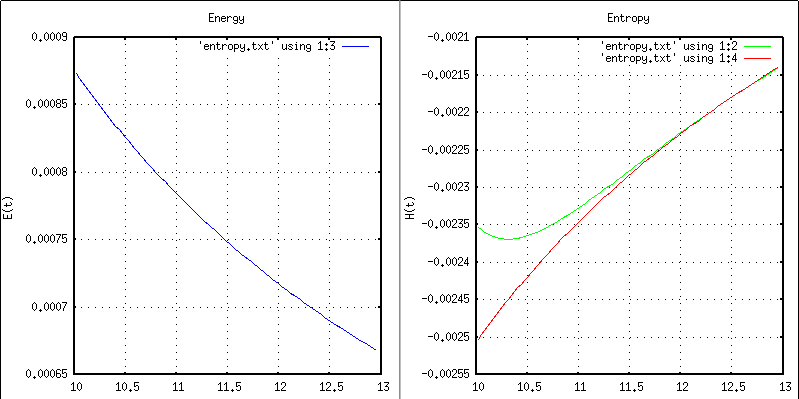
\includegraphics[scale=0.5]{entropy_expansion}

We would also like a good way to check the power with which the energy
density is changing, because of equation 26. We know the energy density
should fall off with a slope of $-\frac{2}{n}$ on a log-log plot.
We can check what power the energy density slope falls off with by
looking at the slope between two different points in time on a plot
of $log(\rho)\, vs\, log(T)$. However, this requires us to store
the data from previous time steps such that we can compare old energy
densities with the most recent. The code in {[}6{]} requires that
we initialize arrays of a size proportional to the total time the
simulation will be run in order to store the energy values for the
entirety. Then the values of the energy density and $\tau$ are stored
in separate arrays, labeled as Energy{[}{]} and Time{[}{]} in the
algorithm below. The slope of the line in the $log(\rho)\, vs\, log(T)$
plot is found by the classic formula

\[
m_{\rho}=\frac{log(\rho_{old})-log(\rho_{current})}{log(T_{old})-log(T_{current})}
\]


The subscript ``old'' and ``current'' refers to the iterative
time step. This poses a problem because traditionally the iterators
would be integers that increase by 1 every time step. If we set the
old time step to a constant, we have to wait for the simulation to
hit that time step to start to gain useful slope information, and
then the estimate gets less and less accurate as $t\gg t_{0}$. Instead,
we'd like to track the most recent slope. Again, we could use the
current time-step plus or minus a constant, but the same problem arises
at large t due to the logarithm. Instead, let's define a new quantity
L, which will be a constant, and the current time step, t. The most
recent slope can be tracked by taking L\textasciitilde{}1. If we increase
L from 1.0 to 1.3, we've effectively changed the range of the most
recent slope calculation. So this allows an easy way to adjust how
far back we want to judge the slope. This becomes useful because the
real-world time it takes for $m_{\rho}$ to converge on $-\frac{2}{n}$
is proportional to the step size $\triangle t$. It is then useful
to use only the most recent piece of the line from the log-log plot
to determine the value of $m_{\rho}$. 

\begin{algorithm}[!h]
\begin{algor}
\item [{while}] $(t<t_{max})$
\item [{{*}}] $L=1.1$
\item [{{*}}] $m_{\rho}=\frac{log(Energy[floor(\frac{t}{L})])-log(Energy[t])}{log(Time[floor(\frac{t}{L})])-log(Time[t])}$
\item [{endwhile}]~
\end{algor}
\caption{Track recent slope on log-log plot}


\end{algorithm}


Notice the use of the floor() function in Algorithm 23. The floor(x)
function returns the lowest integer for a given x. We could have just
as easily used the ceil() function without effecting the outcome of
the slope calculation.

Now probing different eras (n=2,3,4...etc) should result in log-log
plots which are linear with a slope of $m_{\rho}=-\frac{2}{n}$. This
will be a strong indication that the gravitational terms calculated
in the previous sections are working correctly.


\section{Loop Tracking and Removal}

We would like to now understand how loop production affects the distribution.
To do so, we will present a method of loop removal such that we can
track how much energy density goes into large and small loops, respectively.
To begin, we assume that f(A,B) is a distribution of long strings.
The long strings radiate loops due to self-intersecting wiggles and
string inter-commutation. We will modify the transport equation (4)
such that certain conditions will lead to the removal of string segments,
which in turn removes energy density from the distribution. The removed
energy density will be stored just like we did for the collision term,
but we'll separate it into two new arrays, one for small loops, and
one for large loops. Also, to keep the transport equation equivalent
to what we did in Part 1 and 2, whenever we remove loops from the
distribution, we'll also track what was removed and how much. Then
we will add all of these back into the original distribution, effectively
leaving the transport equation and distribution function unchanged.
However, we will now be able to track the energy density present due
to small, large, and red-shifted loops, as well as that due to long
strings. Recall the original transport equation: 
\[
\left(\frac{df}{dt}\right)_{collision}=\frac{1}{\rho}\int\, d\mathbf{A}'d\mathbf{B}'\,\Gamma\left(\, f(\mathbf{A}',\mathbf{B})f(\mathbf{A},\mathbf{B}')-f(\mathbf{A},\mathbf{B})f(\mathbf{A}',\mathbf{B}')\,\right)
\]


Or in terms of the Lebedev quadrature, with gamma expanded:

\[
\left(df(A,B)\right)_{col}=\sum_{A'=0}^{n}\sum_{B'=0}^{n}\frac{1}{\rho}\, w_{A'}w_{B'}\,(\lambda(\frac{1}{\mu})+p\rho\mu P(A,B,A',B'))\left(\, f(A',B)f(A,B')-f(A,B)f(A',B')\,\right)\Delta t
\]


We will now separate the above equation into two separate equations,
one for small loops and one for large. Each of these will tell us
about the change in energy density due to collisions among their corresponding
types of string segments. 

The conditions for loop removal are two-fold. There are two different
types of loops, small and large. Due to the $\Gamma$ term, the equation
is repeated twice and summed together. One is proportional to the
probability $\lambda$, and the other is proportional to $pP(A,B,A',B')$,
where p is the inter-commutation probability. These two parts of gamma
correspond to small loop production and large loop production from
inter-commutation. So only large loops depend on inter-commutation.
In section 1.1 we set $\lambda=1$. Now we will leave it as a tunable
parameter. Then we can break up collision term into two separate terms. 

\begin{equation}
\left(df(A,B)\right)_{small}=\sum_{A'=0}^{n}\sum_{B'=0}^{n}\frac{1}{\rho}\, w_{A'}w_{B'}\,(\lambda(\frac{1}{\mu}))\left(\, f(A',B)f(A,B')-f(A,B)f(A',B')\,\right)\Delta t
\end{equation}


\begin{equation}
\left(df(A,B)\right)_{large}=\sum_{A'=0}^{n}\sum_{B'=0}^{n}w_{A'}w_{B'}\,(\mu pP(A,B,A',B'))\left(\, f(A',B)f(A,B')-f(A,B)f(A',B')\,\right)\Delta t
\end{equation}


We will also need to track the changes in the distribution of long
strings. This term will be modified in two parts as well, one for
when small loops are removed, and one for when large loops are removed.
These correspond (as in 38 and 39) to the side with $\lambda$ dependence,
and the side with P dependence. 

\[
\left(df(A,B)\right)_{long}=\left(df(A,B)\right)_{long\,(small)}+\left(df(A,B)\right)_{long\,(large)}
\]


Which splits up in terms of quadrature like:

\begin{equation}
\left(df(A,B)\right)_{long\,(small)}=\sum_{A'=0}^{n}\sum_{B'=0}^{n}\frac{1}{\rho}\, w_{A'}w_{B'}\,(\lambda(\frac{1}{\mu}))\left(\, f(A',B)f(A,B')\right)\Delta t
\end{equation}


\begin{equation}
\left(df(A,B)\right)_{long\,(large)}=\sum_{A'=0}^{n}\sum_{B'=0}^{n}w_{A'}w_{B'}\,(\mu pP(A,B,A',B'))\left(\, f(A',B)f(A,B')\right)\Delta t
\end{equation}



\subsection{Small Loop Production}

Small loops are the smallest possible closed collection of unit vectors
A, B, A' and B' that the system allows. This occurs when $\mathbf{u}=-\mathbf{u}'$.
Because \textbf{u} is defined in terms of \textbf{A} and \textbf{B,}
and these vectors are perpendicular to one another, we can define
a closed loop as follows.

\begin{equation}
B+B'-A-A'=0
\end{equation}


Graphically, we can think of these string segments as unit vectors
connecting at their ends to form a loop. 

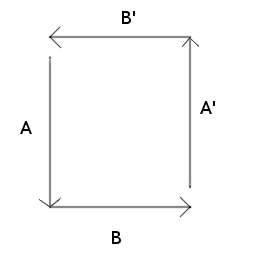
\includegraphics[scale=0.5]{abapbp}

The distribution of small loops is then comprised only of distributions
of f(A,B) and f(A'B'). If we detect a loop, (e.g. equation 42 is true),
we set $f(A,B)f(A',B')=0$, such that we have:

\begin{equation}
df(A,B)_{small}=\frac{1}{\rho}\int d\mathbf{A}'d\mathbf{B}'(0-f(\mathbf{A},\mathbf{B})f(\mathbf{A}'\mathbf{B}')
\end{equation}


A simple if() statement can handle the small loops removal condition.
We also track how much of the long string distribution we set to zero
when the if() statement was true. The algorithm to remove loops then
goes as follows.

\begin{algorithm}[!h]
\begin{algor}
\item [{for}] \ensuremath{(A=0;\, A<N;\, A++)}


\begin{algor}
\item [{for}] $(B=0;\: B<N;\: B++)$

\begin{algor}
\item [{for}] \ensuremath{(A=0;\, A<N;\, A++)}


\begin{algor}
\item [{for}] $(B=0;\: B<N;\: B++)$
\item [{{*}}] $F=f[A'][B]f[A][B']$
\item [{if}] $(|(Point[B]+Point[B']-Point[A]-Point[A'])|\leq CUTOFF)$
\item [{{*}}] $F=0$
\item [{{*}}] $df_{long(small)}[A][B]=df_{long(small)}[A][B]+\frac{1}{\rho}\,(\lambda)\left(\, f[A'][B]f[A][B']\right)\, Point[A'].GetWeight()\, Point[B'].GetWeight()\Delta t$
\item [{endif}]~
\item [{{*}}] $df_{small}[A][B]=df_{small}[A][B]+(\frac{1}{\rho})\,(\lambda)(F-f[A][B]f[A'][B'])\, Point[A'].GetWeight()\, Point[B'].GetWeight()\Delta t$ 
\item [{endfor}]~
\end{algor}
\item [{endfor}]~
\end{algor}
\item [{endfor}]~
\end{algor}
\item [{endfor}]~
\end{algor}
\caption{Calculate the probability density of small loops $\left(df(A,B)\right)_{small}$}
\end{algorithm}


Notice that the term CUTOFF is set at runtime, and the the quantity
|(Point{[}B{]}+Point{[}B'{]}-Point{[}A{]}-Point{[}A'{]})| represents
the magnitude of the resulting vector. The amount of the distribution
that is removed due to small loops will obviously be sensitive to
this parameter if it is set to high. It needs to be a good numerical
approximation to zero on the machine which the code is run on. In
our simulations from {[}6{]}, $CUTOFF=10^{-12}$. 


\subsection{Large Loop Production}

In the same way we now want to remove any other segments that are
loops, so long as they are greater than the small loops cutoff. These
we call large loops. They again come from the term f(A,B)f(A',B'),
so we want to set the term f(A',B)f(A,B') to zero if the condition
is true. So we again have an if() statement that will determine whether
or not a large loop is produced.

\begin{equation}
B+B'-A-A'>CUTOFF
\end{equation}


If (46) is true, then our formula for the changes in the distribution
due to interactions of large loops goes like:

\begin{equation}
df(A,B)_{large}=\int d\mathbf{A}'d\mathbf{B}'(0-f(\mathbf{A},\mathbf{B})f(\mathbf{A}'\mathbf{B}')
\end{equation}


And at the same time, we calculate $df_{long(large)}$ to account
for what we removed. Notice that the $\rho$ cancels. Then the algorithm
goes like one would expect:

\pagebreak{}

\begin{algorithm}[!h]
\begin{algor}
\item [{for}] \ensuremath{(A=0;\, A<N;\, A++)}


\begin{algor}
\item [{for}] $(B=0;\: B<N;\: B++)$

\begin{algor}
\item [{for}] \ensuremath{(A=0;\, A<N;\, A++)}


\begin{algor}
\item [{for}] $(B=0;\: B<N;\: B++)$
\item [{{*}}] $F=f[A'][B]f[A][B']$
\item [{if}] $(|(Point[B]+Point[B']-Point[A]-Point[A'])|>CUTOFF)$
\item [{{*}}] $F=0$
\item [{{*}}] $df_{long(large)}[A][B]=df_{long(large)}[A][B]+(pP[A][B][A'][B'])\left(\, f[A'][B]f[A][B']\right)\, Point[A'].GetWeight()\, Point[B'].GetWeight()\Delta t$
\item [{endif}]~
\item [{{*}}] $df_{large}[A][B]=(pP[A][B][A'][B'])(F-f[A][B]f[A'][B'])\, Point[A'].GetWeight()\, Point[B'].GetWeight()\Delta t$ 
\item [{endfor}]~
\end{algor}
\item [{endfor}]~
\end{algor}
\item [{endfor}]~
\end{algor}
\item [{endfor}]~
\end{algor}
\caption{Calculate the probability density of large loops $\left(df(A,B)\right)_{large}$}
\end{algorithm}


The first thing you will notice is that these changes in the distributions
are all negative, with the exception of $df(A,B)_{long}$. So adding
the large and small loops terms removes energy density from the distribution
and the long strings term adds energy back in. We can treat these
terms as proper distribution functions all on their own, which obey
all the familiar rules, such that we can still calculate energy density,
pressure, and entropy. 

Updating the distribution function as before will lead to the same
results as we had in Section 1 and 2 because we've essentially just
set up a means of tracking where energy goes. Add the removed probability
density back into the distribution as always, but now replace $df_{coll}[A][B]$
with $df_{small}[A][B]+df_{large}[A][B]+df_{long}[A][B]$. 

\begin{algorithm}[!h]
\begin{algor}
\item [{for}] \ensuremath{(A=0;\, A<N;\, A++)}


\begin{algor}
\item [{for}] $(B=0;\: B<N;\: B++)$

\begin{algor}
\item [{{*}}] $f[A][B]=f[A][B]+df_{small}[A][B]+df_{large}[A][B]+df_{long}[A][B]+df_{g}[A][B]$ 
\end{algor}
\item [{endfor}]~
\end{algor}
\item [{endfor}]~
\end{algor}
\caption{Track large and small loops in distribution function}
\end{algorithm}


One can verify that the distribution function has not been changed
by integrating over it and looking at a log-log plot of the energy
density with time, as was shown in section 2.7. The same results should
hold. The energy density falls off as $\rho\propto t^{-\frac{2}{n}}$,
where n=2 for curvature, n=3 for matter, and n=4 for radiation dominated
universes. However, in the next section we will stop adding back the
energy density due to long strings that is lost when loops are removed.


\subsection{Ratio of Small to Large Loops}

Now we would like to see how the distribution behaves when we actually
remove large and small loops from the distribution. Simply remove
the quantity $df_{long}[A][B]$ from the update function given in
Algorithm 26. The slope of $log(\rho)$ vs $log(t)$ should go to
-2. 

\begin{algorithm}[!h]
\begin{algor}
\item [{for}] \ensuremath{(A=0;\, A<N;\, A++)}


\begin{algor}
\item [{for}] $(B=0;\: B<N;\: B++)$

\begin{algor}
\item [{{*}}] $f[A][B]=f[A][B]+df_{small}[A][B]+df_{large}[A][B]+df_{g}[A][B]$ 
\end{algor}
\item [{endfor}]~
\end{algor}
\item [{endfor}]~
\end{algor}
\caption{Remove large and small loops from the distribution function}
\end{algorithm}
We are now set to define a few other quantities. The energy density
which has been removed due to small loop production at each time step
can be calculated like:

\begin{equation}
\rho_{small}=\int\,\left(df(A,B)_{small}\right)dA\, dB
\end{equation}


And likewise for large loops:

\begin{equation}
\rho_{large}=\int(df(A,B)_{large})dA\, dB
\end{equation}


As well as red-shifted loops:

\begin{equation}
\rho_{redshift}=\int(df(A,B)_{g})dA\, dB
\end{equation}


These can be calculated in the usual way with the Lebedev Quadrature
according to equation 6. With these quantities we can construct the
ratio between small and large loops, $\ell$.

\begin{equation}
\ell=\frac{\rho_{small}}{\rho_{large}}
\end{equation}


We must also define the correlation length $\mu$, which we had set
to 1 in the previous sections. We must calculate this quantity dynamically.
The definition is recursive, so the current value $\mu$ is defined
in terms of the value at the previous time step $\mu_{0}$:

\[
\mu=\mu_{0}(1+x\left(\frac{\rho_{small}}{\rho}\right)+y\left(\frac{\rho_{large}}{\rho}\right)+z\left(\frac{\rho_{redshift}}{\rho}\right))
\]


We'll define the energy densities $\rho_{small}$, $\rho_{large}$
and $\rho_{redshift}$ in section 3.3. The coefficients in front of
these terms are constants which obey the following constraints.

\[
x<-\frac{1}{2}
\]


\[
y>0
\]


\[
z<0
\]


\[
\gamma=\frac{\mathcal{H}}{\tau}
\]


Then we can define predicted values for the energy densities $\rho_{small}$,
$\rho_{large}$ and $\rho_{redshift}$ in terms of x, y, and z. We
call them A, B, and C respectively.

\[
A+B+C=1
\]


Through numerical simulation, we have found that the ratio of small
to large loops can be described in terms of x, y, and z in Minkowski
space (i.e. z=0) as follows:

\[
A=\frac{1+2y}{2y-2x}
\]


\[
B=\frac{1+2x}{2x-2y}
\]


\[
\ell=\frac{A}{B}
\]

\begin{thebibliography}{1}
\bibitem{key-1}V. Vanchurin, ``Towards a kinetic theory of strings'',
arXiv:1103.1593v3 {[}hep-th{]} (May, 2011)

\bibitem{key-2}D. Schubring and V. Vanchurin, ``Fluid Mechanics
of Strings'', arXiv:1305.6961v2 {[}hep-th{]} (June 2013)

\bibitem{key-3}D. Schubring and V. Vanchurin, ``Transport Equation
for Nambu-Goto Strings'' arXiv:1310.6763v1 {[}hep-th{]} (October
2013)

\bibitem{key-6}V.Vanchurin, ``Kinetic Theory and Hydrodynamics of
Cosmic Strings'', arXiv:1301.1973v3 {[}hep-th{]} (March 2013)

\bibitem{key-8} John Burkhard's Lebedev Quadrature rules, ``http://people.sc.fsu.edu/\textasciitilde{}jburkardt/datasets/sphere\_lebedev\_rule/sphere\_lebedev\_rule.html''

\bibitem{key-8-1} Jacob Balma, ``Code: http:73.164.34.35/c\_projects/''

\bibitem{key-1}MB Hindmarsh and T W B Kibble, ``Cosmic Strings'',
Rep. Prog. Phys. 1 February, 2008

\bibitem{key-1}William H. Press, ``Numerical Recipes in C++'',
Cambridge Press, 2005\end{thebibliography}

\end{document}
